\documentclass[a4paper,11pt]{ltjsarticle}

\usepackage{luatexja}
\usepackage{geometry}
\geometry{margin=25mm}

\usepackage{array}
\usepackage{longtable}
\usepackage[table]{xcolor}
\usepackage{booktabs}

\usepackage{enumitem}

\usepackage{hyperref}

\usepackage{titlesec}
\titleformat{\section}{\large\bfseries}{\thesection.}{0.5em}{}

\usepackage{listings}
\lstset{
  basicstyle=\ttfamily\small,
  frame=single,
  breaklines=true,
  numbers=left,
  numberstyle=\tiny\color{gray},
  keepspaces=true,
  showstringspaces=false,
  columns=fullflexible,
  tabsize=2,
}

\usepackage{tikz}
\usetikzlibrary{shapes.geometric, arrows.meta, positioning, calc, fit}

\usepackage{graphicx}

\usepackage{float}

\definecolor{ganttCell}{HTML}{4FC3D0}
\definecolor{ganttEarly}{HTML}{FFB74D}

\providecommand{\％}{\%}

\setlength{\parindent}{0pt}
\setlist[itemize]{leftmargin=2em}

% 表セル内のコード識別子(LOOP_REST_TICKS等)が長く改行できない場合の救済。
\setlength{\emergencystretch}{6em}

\begin{document}

\begin{center}
    {\LARGE \textbf{第9回事前課題}}\\[0.4em]
    {\large 作業ログ（第8週末）}\\[1em]
\end{center}

\begin{tabular}{|p{4cm}|p{10cm}|}
\hline
報告者 & 櫛濱 和輝 (25G1046)\\
\hline
報告日 & 2026年6月23日\\
\hline
チーム & チーム9\\
\hline
プロジェクト名 & 赤外線通信で歌うカエル\\
\hline
担当パート & 親機と子機の赤外線通信（輪唱機能作成）：親機ファーム hack-oya.ino（計画書 v1.1 の master.ino に対応），子機ファーム hack-ko.ino（同 child\_xxx.ino に対応），両者を媒介する Processing 側 hackko.pde の休符処理，および親機回路（子機ボタン群／状態表示 LED ／ start ボタン）の組み立て\\
\hline
本来の今週の位置づけ & 第8週末（6/23）．計画書 v1.1（2026/6/19版）のガント上，第8週は 510:結合テストの実施期間．櫛濱はチーム作業ログ v6/19版「次回予定（第9週）」に挙げられた「新しい親機側のコード作成」を引き取り，親機⇔子機の赤外線通信プロトコル整備と複数子機輪唱の実機完成を担当\\
\hline
報告対象 & 前回個人作業ログ（6/16）以降に実施した\textbf{親機と子機の赤外線通信による輪唱機能の実機完成}．具体的には親機回路の組み立て（子機ボタン D4--D7／状態表示 LED A0--A3／start ボタン D8），親機ファーム（hack-oya.ino）の押下順カノン entry 動的割当・誤操作ガード・チャタリング対策，子機ファーム（hack-ko.ino）の親機との周期 TICK\_LENGTH 整合，Processing（hackko.pde）の休符即時停止\\
\hline
作業時間 & 計10時間\\
\hline
\end{tabular}

\vspace{1em}

%=====================================================
\section{進捗サマリー}\label{sec:summary}

\begin{itemize}
    \item 現在地：第8週末（6/23）．チーム作業ログ v6/19版時点では「ドラムを除く 3 楽器での輪唱開始は確認できた」状態で，ドラムを含む 4 子機（ピアノ・フルート・トランペット・ドラム）の同時稼働と，輪唱方針見直しに対応した親機ファーム再実装が「次回予定（第9週）」として残されていた．今週これを引き取り完了させた
    \item \textbf{親機 hack-oya.ino（計画書の master.ino に対応）の主要実装}：
    \begin{itemize}
        \item NEC プロトコルによる単一ブロードキャスト方式を実装．アドレス上位 8bit に cyclePos，下位 8bit に enabledMask（各子機が今 tick で鳴るかのビット集合），コマンド上位 2bit に configIdx，下位 6bit に canonOffset を載せて 1 フレームで全子機へ一斉送出する
        \item 子機ボタン（D4--D7）の隣にトグル状態表示 LED（A0--A3）を追加し，どの子機が参加予約／参加中なのかを物理 UI で可視化．従来は親機 Serial Monitor を見ないと状態が分からなかった
        \item start ボタン（D8）に「子機が 1 つも選択されていない状態では演奏を開始しない」ガードを追加し，無音 tick を撒き続ける誤操作を防止
        \item ボタン入力を \texttt{delay(30)} 方式から \texttt{millis()} ベースの状態継続式 debounce（同じ生値が 50ms 続いたら確定）に置換．長押し中の瞬間バウンスによる二重トグル発火を抑止
        \item \textbf{押下順カノン entry 動的割当}：従来 \texttt{CHILD\_ENTRY[i]=\{0,8,16,20\}} を子機固有値として扱っていたが，これを \texttt{CANON\_ENTRY\_BY\_ORDER} に再解釈し，押下順 N 番目に対して 0, 8, 16, 20 を割り当てる方式に変更．どのボタンを最初に押してもその子機が pos0 から流れ出し，2 番目以降が 8, 16, 20 tick 遅れて参加する本来のカノン形になった
    \end{itemize}
    \item \textbf{子機 hack-ko.ino（計画書の child\_xxx.ino に対応）の修正}：親機側 \texttt{LOOP\_REST\_TICKS=1}（TICK\_LENGTH=32）に対し子機側が 2（TICK\_LENGTH=33）のまま残っており，ループ折り返しで子機 \texttt{localPos = (cyclePos - myOffset + 33) \% 33} が 1tick 飛ぶ症状（child2 で pos16，child1 で pos24 が抜ける）が発生していた．子機側 \texttt{LOOP\_REST\_TICKS} を 1 に揃え，両者の周期を 32 に統一して根絶
    \item \textbf{Processing hackko.pde の修正}：\texttt{NOTE\_DURATION\_DEFAULT=0.40s} が tick 間隔（120BPM で 0.25s）より長く，R（休符）の tick でも前音の余韻が次拍まで残り休符として聞こえない症状があった．\texttt{PianoInstrument currentInstrument} を保持しておき，R 受信時に \texttt{noteOff()} で即停止することで休符を聴感上機能させた
    \item 全体進捗率：チーム作業ログ v6/19版で 510:結合テスト 50\%（ドラム除く 3 楽器の輪唱開始確認）だったところを，ドラム込み 4 子機の輪唱演奏まで進めた．残課題は MOP1 演奏タイミング誤差の定量計測・MOP2 同期信号受信成功率（95\% 目標）の定量計測・MOP4 音色再現性アンケート・MOP5 歌詞アニメーション同期遅延（LCD 担当範囲）
    \item 主要成果：
    \begin{itemize}
        \item \textbf{親機 1 台と 4 子機（ピアノ・フルート・トランペット・ドラム）による赤外線通信輪唱が実機で稼働した}．押下順に従ったカノン演奏を聴感で確認
        \item 親機回路に物理 UI（トグル LED ・ start ボタン）を実装し，リハーサル時の操作性が大きく向上．Serial Monitor を見ずに「どの子機を参加させたか」「いま再生中か」が判別できる状態になった
        \item 親機・子機間の TICK\_LENGTH 不整合という長期間潜伏していたバグを発見・修正．以後 pos16／pos24 抜けの再発なし
    \end{itemize}
    \item 重大課題（影響度：高）：
    \begin{itemize}
        \item 子機 hack-ko.ino の双子音処理（\texttt{DOUBLE\_START=24} 以降の半 tick 区間）に \texttt{delay(lastIntervalMs/2)} が残っており，その間 IR 受信ループが止まる．pos25 付近の取りこぼし要因として残存．\texttt{millis()} ベースの遅延発火に置換予定
        \item チーム作業ログ v6/19版で計画書側にも記載された MOP2「同期信号の受信成功率 95\% 以上」は依然定量未計測．第9週に 4 子機分の送受信ログから算出する
        \item 計画書 v1.1 で導入された OFF / QUEUED / ACTIVE 状態管理は，本実装では \texttt{canonOffset[]}（参加中の遅延値，-1 で不参加）／\texttt{pendingOffset[]}（予約済み．\texttt{cyclePos} 一致時に \texttt{canonOffset} へ昇格）の 2 配列で等価機能を実現している．状態名の対応関係は次節以降に明記する
    \end{itemize}
\end{itemize}

%=====================================================
\section{ガントチャート}\label{sec:gantt}

第8週末時点では計画書 v1.1（2026/6/19版）から変更はないため，チーム全体・個人とも v1.1 のガントチャートのみを掲載する．着色セル（\colorbox{ganttCell}{\phantom{xx}}）は当該タスクの実施週を表す．

\renewcommand{\arraystretch}{1.3}

\begingroup
\setlength{\tabcolsep}{3pt}

\subsection{チーム全体ガントチャート}\label{sec:gantt-team}

\begin{longtable}{|p{6.2cm}|p{2.3cm}|c|c|c|c|c|c|}
\hline
\rowcolor[gray]{0.9}
第3層：活動タスク & 担当者 & 5週 & 6週 & 7週 & 8週 & 9週 & 10週 \\
\hline
110:ピアノ音の作成 & 櫛濱・久家 & \cellcolor{ganttCell} & & \cellcolor{ganttCell} & & & \\
\hline
120:arduinoとの通信用関数（ピアノ） & 櫛濱・久家 & \cellcolor{ganttCell} & & & & & \\
\hline
130:フルート音の作成 & 家田 & \cellcolor{ganttCell} & & & & & \\
\hline
140:arduinoとの通信用関数（フルート） & 家田 & \cellcolor{ganttCell} & & & & & \\
\hline
150:トランペット音の作成 & 木下 & \cellcolor{ganttCell} & & & & & \\
\hline
160:arduinoとの通信用関数（トランペット） & 木下 & \cellcolor{ganttCell} & & & & & \\
\hline
170:ドラム音の作成（キック） & 久家 & & \cellcolor{ganttCell} & & & & \\
\hline
171:ドラム音の作成（シンバル） & 久家 & & \cellcolor{ganttCell} & & & & \\
\hline
180:arduinoとの通信用関数（ドラム） & 久家 & & \cellcolor{ganttCell} & & & & \\
\hline
210:ピアノのプログラム & 櫛濱 & \cellcolor{ganttCell} & & & & & \\
\hline
220:フルートのプログラム & 家田 & \cellcolor{ganttCell} & & & & & \\
\hline
230:トランペットのプログラム & 木下 & \cellcolor{ganttCell} & & & & & \\
\hline
240:ドラムのプログラム & 久家 & & \cellcolor{ganttCell} & & & & \\
\hline
250:楽譜進行プログラム & 渡邊 & & \cellcolor{ganttCell} & \cellcolor{ganttCell} & \cellcolor{ganttCell} & & \\
\hline
310:赤外線管理プログラム & 家田・渡邊 & & \cellcolor{ganttCell} & \cellcolor{ganttCell} & \cellcolor{ganttCell} & & \\
\hline
320:テンポ管理プログラム & 渡邊 & & \cellcolor{ganttCell} & & & & \\
\hline
410:回路作成 & 手代木 & & \cellcolor{ganttCell} & & & & \\
\hline
420:LEDマトリクス作成 & 手代木 & & \cellcolor{ganttCell} & \cellcolor{ganttCell} & \cellcolor{ganttCell} & & \\
\hline
510:結合テスト & 全員 & & & & \cellcolor{ganttCell} & \cellcolor{ganttCell} & \cellcolor{ganttCell} \\
\hline
\end{longtable}

\endgroup

\subsection{個人ガントチャート（計画書 v1.1 から櫛濱担当分を抜粋）}\label{sec:gantt-personal}

\ref{sec:gantt-team} 節のチーム全体ガントから櫛濱担当分（櫛濱・全員）を抜き出した個人計画．第8週は 510:結合テストの実施期間．本週は親機⇔子機の赤外線通信プロトコル（NEC 単一ブロードキャスト）と発音経路の整備により，4 子機（ピアノ・フルート・トランペット・ドラム）の輪唱を実機で稼働させた．

\begingroup
\setlength{\tabcolsep}{3pt}
\begin{longtable}{|p{0.9cm}|p{2.0cm}|p{5.2cm}|c|c|c|c|c|c|}
\hline
\rowcolor[gray]{0.9}
管理 & 第2層 & 第3層タスク & 5週 & 6週 & 7週 & 8週 & 9週 & 10週 \\
\hline
110 & 100 (Processing) & ピアノ音の作成 & \cellcolor{ganttCell} & & \cellcolor{ganttCell} & & & \\
\hline
120 & 100 (Processing) & arduinoとの通信用関数（ピアノ） & \cellcolor{ganttCell} & & & & & \\
\hline
170 & 100 (Processing) & ドラム音の作成（キック） & & \cellcolor{ganttCell} & & & & \\
\hline
210 & 200 (子機) & ピアノのプログラム & \cellcolor{ganttCell} & & & & & \\
\hline
510 & 500 (包括) & 結合テスト（全員） & & & & \cellcolor{ganttCell} & \cellcolor{ganttCell} & \cellcolor{ganttCell} \\
\hline
\end{longtable}
\endgroup

\subsection{今週の作業位置づけ}\label{sec:gantt-position}

\begin{itemize}
    \item 現在地は第8週末（6/23）．GC 上，第8週は 510:結合テストの実施期間．チーム作業ログ v6/19版時点でドラム除く 3 楽器の輪唱開始は確認できていたが，ドラムを含む全 4 子機の輪唱と，計画書 v1.1 で導入された「OFF / QUEUED / ACTIVE による小節頭開始予約」相当の動作（本実装では \texttt{canonOffset[]} ／ \texttt{pendingOffset[]} の 2 配列で実現）が未実装だった．本週でこれらをすべて完了させた．
    \item 親機回路を組み上げ，子機ボタン D4--D7／状態表示 LED A0--A3／start ボタン D8 を整備．Serial Monitor を見なくても運用できる物理 UI を確保した．
    \item 親機ファーム hack-oya.ino と子機ファーム hack-ko.ino の間で長期間潜伏していた TICK\_LENGTH 不一致（親 32／子 33）を発見・修正し，特定 localPos が周期的に抜ける症状を根絶．
    \item 次週以降は 510:結合テスト本体の定量フェーズに入り，MOP1 演奏タイミング誤差・MOP2 赤外線通信成功率の定量計測，および双子音処理の非ブロック化を進める．
\end{itemize}

%=====================================================
\section{作業ログ}\label{sec:worklog}

\renewcommand{\arraystretch}{1.4}

\begingroup
\setlength{\tabcolsep}{3pt}
\sloppy
{\footnotesize
\begin{longtable}{|p{2.6cm}|p{1.1cm}|p{1.3cm}|p{1.0cm}|p{0.9cm}|p{2.2cm}|p{4.5cm}|}
\hline
\rowcolor[gray]{0.9}
作業項目 & 開始日 & 予定完了日 & 状態 & 進捗率 & 依存関係・ブロッカー & コメント \\
\hline
親機回路の組み立て（子機ボタン横 LED ／ start ボタン） & 6/17 & 6/19 & 完了 & 100\％ & D4--D7 ボタン／A0--A3 LED／D8 start ボタン & ブレッドボード上で子機ボタンの隣に LED を配置．D4--D7 と中央溝をまたいだ向こう側に A0--A3 から各 LED アノードを配線．\textbf{ボタン操作中も状態が一目で分かる UI} になり，運用性が大幅向上 \\
\hline
ボタン入力の debounce 強化（hack-oya.ino） & 6/19 & 6/20 & 完了 & 100\％ & 物理ボタンのバウンス特性 & \texttt{delay(30)} 方式から \texttt{millis()} ベースの状態継続式（50ms 安定継続で確定）に置換．長押し中の瞬間バウンスで二重 toggle 発火する症状を解消 \\
\hline
start 空打ち抑止（hack-oya.ino） & 6/20 & 6/20 & 完了 & 100\％ & start ボタン UI／canonOffset・pendingOffset 管理 & 子機が 1 つも選択されていない（canonOffset／pendingOffset 全 -1）状態で start を押しても \texttt{isPlaying} に遷移しないガードを追加 \\
\hline
親機⇔子機 TICK\_LENGTH 整合（hack-ko.ino） & 6/22 & 6/22 & 完了 & 100\％ & 親機側 \texttt{LOOP\_\-REST\_\-TICKS=1} & 子機側 \texttt{LOOP\_\-REST\_\-TICKS} を 2→1 に揃え，両者の TICK\_LENGTH を 32 に統一．child2 で pos16，child1 で pos24 等の特定 localPos が抜ける症状を根絶 \\
\hline
押下順カノン entry 動的割当（hack-oya.ino） & 6/22 & 6/22 & 完了 & 100\％ & 既存 CHILD\_ENTRY 設計 & \texttt{CHILD\_ENTRY[i]} を子機固有値から「押下順 N 番目に割り当てる遅延値」 \texttt{CANON\_ENTRY\_BY\_ORDER[order]} に再解釈．どのボタンを最初に押してもその子機が pos0 から流れ出すよう動的割当に変更 \\
\hline
休符 R の即時 noteOff（hackko.pde） & 6/22 & 6/22 & 完了 & 100\％ & PianoInstrument の保持 & \texttt{NOTE\_DURATION\_DEFAULT=0.40s} が tick 間隔より長く R が休符に聞こえない症状を，R 受信時の \texttt{noteOff()} 即時停止で解消 \\
\hline
4 子機輪唱の実機テスト & 6/23 & 6/23 & 完了 & 100\％ & 親機ファーム／子機ファーム×4／hackko.pde／drum.pde & 親機 1 台＋子機 4 台（ピアノ・フルート・トランペット・ドラム）の構成で，押下順カノンと TICK\_LENGTH 整合後の輪唱演奏を聴感で確認．pos 抜け・休符抜けの再発なし \\
\hline
\end{longtable}
}
\endgroup

%=====================================================
\section{評価事項}\label{sec:evaluation}

計画書 v1.1（2026/6/19版）「1.4 検証と妥当性確認: V\&V 計画」のうち，今週の作業（輪唱実機統合・親機 UI 改良・各種ファーム修正）に対応する項目を整理する．

\subsection{対応する有効指標 MOE}\label{sec:moe}

\begin{longtable}{|p{1.2cm}|p{4cm}|p{8cm}|}
\hline
\rowcolor[gray]{0.9}
No. & MOE & 評価基準 \\
\hline
MOE1 & 違和感なく聞くことができる & 「かえるのうた」の輪唱が，聴衆が聴いてズレを感じることなく演奏できている．また，音が意図せず途切れることなく最後まで演奏できる \\
\hline
MOE3 & 楽器音らしい音色である & Processing で合成した音が楽器音として聴衆に認識される \\
\hline
\end{longtable}

\subsection{対応する性能指標 MOP（計画書 v1.1）}\label{sec:mop}

\begin{longtable}{|p{1.2cm}|p{3.8cm}|p{8.8cm}|}
\hline
\rowcolor[gray]{0.9}
No. & 性能指標 & 目標値・評価基準 \\
\hline
MOP1 & 演奏タイミング誤差 & 各演奏側 Arduino 間の音符開始タイミングのズレが 30 ms 以内であること \\
\hline
MOP2 & 同期信号の受信成功率 & 指揮側から送信した赤外線信号を演奏側が正しく受信できる割合が 95\% 以上であること \\
\hline
MOP3 & テンポ変更への追従時間 & 指揮側がテンポを変更してから演奏側全台が新テンポに追従するまでの時間が 1 拍以内であること \\
\hline
MOP4 & 音色の再現性 & 倍音構造・ADSR の設定により，対応する楽器の音色として聴衆の過半数に評価されること \\
\hline
\end{longtable}

\subsection{今週の自己評価}\label{sec:selfeval}

\begingroup
\setlength{\tabcolsep}{3pt}
\sloppy
\begin{longtable}{|p{1.0cm}|p{2.8cm}|p{1.8cm}|p{8.7cm}|}
\hline
\rowcolor[gray]{0.9}
No. & 項目 & 達成状況 & 備考 \\
\hline
MOE1 & 違和感なく聞ける輪唱 & OK & 4 子機（ピアノ・フルート・トランペット・ドラム）の輪唱を実機で確認．押下順カノンにより，最初に押した子機がリードとして pos0 から流れ出し，後続が 8／16／20 tick 遅れで参加 \\
\hline
MOE3 & 楽器音らしい音色 & OK & ピアノ＋ドラムの組合せで楽器音として聴感で認識可能（他楽器は他メンバー担当） \\
\hline
MOP1 & 演奏タイミング誤差 & 暫定OK & 聴感では破綻なし．\textbf{オシロまたは DAW による 30ms 以内の定量計測は未実施}（第9週で対応） \\
\hline
MOP2 & 同期信号受信成功率 & 暫定OK & 4 子機同時受信は確認．\textbf{95\% 目標との定量比較は未実施}（第9週で対応） \\
\hline
MOP3 & テンポ変更追従時間 & 部分対応 & 親機側 tempo ボタンの実装はあるが LED マトリクス連携が未統合 \\
\hline
\end{longtable}
\endgroup

\subsection{今後評価予定の項目（参考）}\label{sec:futureplan}

\begin{itemize}
    \item MOP1：4 子機の音符開始タイミングをシリアルログから算出し，最大ズレが 30ms 以内であることを確認（第9週）
    \item MOP2：4 子機を一定時間動かして送受信ログから成功率を算出（第9週）
    \item MOP4：音色認識テスト（聴衆過半数が各楽器と識別，アンケート進行中）
    \item MOP5：歌詞・アニメーション同期遅延（LCD 担当の手代木氏範囲）
\end{itemize}

%=====================================================
\section{課題管理}\label{sec:issues}

\begingroup
\setlength{\tabcolsep}{3pt}
\sloppy
{\footnotesize
\begin{longtable}{|p{2.6cm}|p{3.2cm}|p{0.9cm}|p{0.9cm}|p{3.4cm}|p{1.3cm}|p{1.3cm}|}
\hline
\rowcolor[gray]{0.9}
課題 & 発生原因 & 影響度 & 優先度 & 対策 & 期限 & 状態 \\
\hline
双子音処理の \texttt{delay()} による IR 取りこぼし & \texttt{DOUBLE\_\-START=24} 以降の半 tick 遅延を \texttt{delay(last\-Interval\-Ms/2)} で実装しており，その間 IR 受信ループが止まる & 高 & 高 & \texttt{millis()} ベースの遅延発火に置換し，loop() を止めない非ブロック化 & 6/30 & 未対応 \\
\hline
赤外線通信成功率が未計測（MOP2） & 95\% 目標との定量比較が未実施 & 高 & 高 & 4 子機分の送受信ログを取得し成功率を算出 & 6/30 & 未対応 \\
\hline
演奏タイミング誤差が未計測（MOP1） & 30ms 目標との定量比較が未実施 & 中 & 中 & シリアルログまたはオシロで各子機の音符開始時刻を取得し最大ズレを算出 & 6/30 & 未対応 \\
\hline
倍速演奏スイッチと LED マトリクスの連携（MOP3 関連） & 親機側 tempo ボタンと LED 表示側で連動未統合 & 中 & 中 & tempo 値変更時に LED マトリクスへ通知する経路を手代木と相談 & 6/30 & 未対応 \\
\hline
\end{longtable}
}
\endgroup

\vspace{0.5em}
※影響度＝プロジェクトへのインパクト\\
※優先度＝対応の緊急性

%=====================================================
\section{AI利用状況と検証}\label{sec:ai}

\subsection{利用内容}\label{sec:ai-use}

\begin{itemize}
    \item 利用目的：親機 UI 強化（LED 追加・start 空打ち抑止），ボタンの debounce 強化，親機⇔子機の TICK\_LENGTH 不整合の特定，押下順カノンへの設計変更，Processing 側での休符即時停止
    \item 入力（プロンプト要旨）：
    \begin{itemize}
        \item 「D4〜D7 のボタンを押したら隣の LED がトグル点灯するようにしたい」「もう一度押したら消える」
        \item 「長押しすると LED がまた点いてしまう（debounce が不十分）」
        \item 「子機ボタンが押されてない時は start で演奏を開始しないようにしたい」
        \item 「輪唱で pos16 / pos21 等が飛ぶ」→ 親機側 TICK\_LENGTH=32 と子機側 33 の食い違いを特定
        \item 「ボタン 3 を最初に押すと pos16 から始まってしまう．最初に押した子機が pos0 から流れてほしい」
        \item 「楽譜上の R が休符に聞こえない（前音の余韻が次拍まで残る）」
    \end{itemize}
    \item 出力概要：
    \begin{itemize}
        \item hack-oya.ino：A0--A3 への LED トグル出力，\texttt{millis()} ベース状態継続式 debounce，start 空打ち抑止，\texttt{CANON\_ENTRY\_BY\_ORDER} と \texttt{pressOrder[]} による押下順カノン
        \item hack-ko.ino：\texttt{LOOP\_REST\_TICKS} を 1 に揃えて親機と TICK\_LENGTH=32 に統一
        \item hackko.pde：\texttt{PianoInstrument currentInstrument} を保持し，R 受信時に \texttt{noteOff()} で即停止
    \end{itemize}
\end{itemize}

\subsection{検証方法}\label{sec:ai-verify}

\begin{itemize}
    \item 検証手法：
    \begin{itemize}
        \item 親機回路上で D4〜D7 を順にトグルし，対応する A0〜A3 LED が押下ごとに点灯／消灯することを目視確認
        \item 長押し操作（数秒間ボタンを押し続ける）で LED 状態が再反転しないことを目視確認
        \item 子機未選択での start 押下で \texttt{[!] no child selected -- press D4-D7 first} がシリアルに出力され \texttt{isPlaying} に遷移しないことを確認
        \item 4 子機（ピアノ・フルート・トランペット・ドラム）の輪唱を実演し，pos16／pos24 など特定 localPos の抜けが解消されていること，R の tick で前音が即停止することを聴感確認
        \item 押下順カノン：D6（child2）を最初に押すと child2 が pos0 から流れ始め，後で押した子機が 8/16/20 tick 遅れて参加することを聴感確認
    \end{itemize}
    \item 参照資料：
    \begin{itemize}
        \item チーム計画書・設計書 v1.1（2026/6/19版）「1.4 検証と妥当性確認」「2.1 機能一覧」「2.2 システム構成図」「3.3 ソフトウェア設計」
        \item チーム変更履歴 v6/19版（OFF / QUEUED / ACTIVE と mask 方式の導入経緯）
        \item チーム作業ログ v6/19版（第8週末時点の進捗：ドラム除く 3 楽器の輪唱開始確認）
        \item IRremote ライブラリ（v4.x，NEC プロトコル）
        \item Minim ライブラリ公式ドキュメント（ddf.minim.ugens：Oscil／Line／Instrument）
    \end{itemize}
    \item 検証手順：
    \begin{enumerate}
        \item 親機（hack-oya.ino）と 4 台の子機（hack-ko.ino，CHILD\_ID=0,1,2,3）を電源投入し，Processing 側で hackko.pde／drum.pde を Run
        \item 任意の順序でボタン D4〜D7 を押し，対応する LED 点灯と Serial Monitor の \texttt{[child N] RESERVED order=...} 出力を確認
        \item start を押して輪唱を開始し，聴感で輪唱が成立すること（pos 抜け・休符の抜けがないこと）を確認
        \item reset で全停止と全 LED 消灯を確認
    \end{enumerate}
\end{itemize}

\subsection{ファクトチェック結果}\label{sec:ai-fact}

\begin{itemize}
    \item 一致点：
    \begin{itemize}
        \item TICK\_LENGTH 不整合の症状（child2 で pos16，child1 で pos24 が抜ける）が手計算（\texttt{localPos = (cyclePos - myOffset + 33) \% 33} に対し親機 cyclePos は 0..31 周期）と一致．修正後は両者 32 に揃い対称に巡回することを確認
        \item 押下順カノンの動作（最初に押した子機が pos0，N 番目が \texttt{CANON\_ENTRY\_BY\_ORDER[N-1]}）が計画書 v1.1「1.1.3 既存の技術とプロジェクトの独自性」のカノン形（リード→追従）と整合
    \end{itemize}
    \item 不一致・疑義：
    \begin{itemize}
        \item 計画書 v1.1 で導入された OFF / QUEUED / ACTIVE 3 状態管理を，本実装では \texttt{canonOffset[]} ／ \texttt{pendingOffset[]} の 2 配列で等価に表現している（OFF=両配列 -1，QUEUED=\texttt{pendingOffset}>=0，ACTIVE=\texttt{canonOffset}>=0）．状態名の対応関係はチーム内で次週共有し，計画書側に追記するか実装側のコメントに加える
        \item 双子音処理の \texttt{delay()} は IR 受信ループを止めるため非ブロック化が必要．第9週で着手
    \end{itemize}
    \item 最終判断：採用（4 子機輪唱の実機稼働という MOE1 の中核到達点として妥当）
    \item 根拠：
    \begin{itemize}
        \item TICK\_LENGTH 不一致を直したことで，これまで「飛ぶ」「抜ける」と表現されていた症状が消え，輪唱が聴感で破綻なく成立した
        \item 親機 UI（LED ＋ start ボタン）と押下順カノンにより，演奏者がカノンの順序を即興で組み立てられる構成になり，運用上の自由度が増した
    \end{itemize}
\end{itemize}

%=====================================================
\section{次回計画}\label{sec:next}

\begin{itemize}
    \item 目標（第9週）：
    \begin{itemize}
        \item 双子音処理の \texttt{delay()} 撤去（\texttt{millis()} ベースの遅延発火に置換）
        \item MOP1：4 子機の音符開始タイミングをシリアルログから算出し，最大ズレが 30ms 以内であることを確認
        \item MOP2：4 子機の送受信ログから赤外線通信成功率を定量算出（95\% 目標との比較）
        \item tempo ボタンと LED マトリクス側の表示連動を確認（MOP3 関連，手代木と連携）
        \item OFF / QUEUED / ACTIVE と \texttt{canonOffset[]} ／ \texttt{pendingOffset[]} の対応関係をチーム内で共有
    \end{itemize}
    \item 達成基準：
    \begin{itemize}
        \item 双子音区間でも IR 取りこぼしがなく，全 localPos が連続して送られていることをログで確認
        \item MOP1 の 30ms 以内・MOP2 の 95\% 以上を数値で提示できること
    \end{itemize}
    \item 期限：
    \begin{itemize}
        \item 6/30（第9週末）
    \end{itemize}
\end{itemize}

%=====================================================
\section{その他}\label{sec:other}

\begin{itemize}
    \item 押下順カノン化に伴い，\texttt{CHILD\_ENTRY} を子機固有値として参照していた他メンバーのコード（家田・渡邊側の楽譜進行プログラム 250）と仕様すり合わせが必要．次週ミーティングで共有する
    \item 親機回路の LED 追加に伴い，配線がブレッドボード中央溝をまたぐ箇所が増えた．配線取り回しを LED の位置を 1〜2 行ずらすことで解消した知見を回路担当（手代木）と共有
    \item 双子音区間の非ブロック化は，子機側の状態管理（pending note と発火時刻）を増やす変更になる．第9週着手前に設計図を更新する
    \item 計画書 v1.1 が言及する LCD キャラクターディスプレイ（カエルの口パクアニメーション・歌詞表示）は手代木担当範囲．LED マトリクス側（420）と統合次第，親機 tempo と表示連動の I/F を相談する
\end{itemize}

%=====================================================
\section{付録}\label{sec:appendix}

\subsection{添付資料}\label{sec:attach}

\begin{itemize}
    \item ソースコード：hack-oya/hack-oya.ino（親機，計画書の master.ino に対応），hack-ko/hack-ko.ino（子機，CHILD\_ID は機体ごとに 0/1/2/3 を設定．計画書の childpiano.ino／childflute.ino／childtrumpet.ino／childdrum.ino を 1 ファイル＋定数差替えで共通化），hackko/hackko.pde（メロディ用 Processing），drum/drum.pde（ドラム用 Processing）
    \item リポジトリ：\url{https://github.com/k-kushihama/hackathon-code/}
\end{itemize}

\subsection{添付範囲}\label{sec:attach-scope}

\begin{itemize}
    \item 第8週に変更した親機ファーム（LED トグル・start 空打ち抑止・debounce・押下順カノン）に該当する hack-oya.ino のスナップショット
    \item 第8週に変更した子機ファーム（TICK\_LENGTH 整合）に該当する hack-ko.ino のスナップショット
    \item 第8週に変更した Processing スケッチ（R 即時 noteOff）に該当する hackko.pde のスナップショット
\end{itemize}

\subsection{システム図}\label{sec:diagrams}

\subsubsection{輪唱システム全体構成}\label{sec:sysdiag}

図~\ref{fig:system} に第8週末時点の輪唱システム全体を示す．親機 1 台（hack-oya.ino）が 4 子機（hack-ko.ino，CHILD\_ID=0〜3）へ NEC フレームを一斉送出し，各子機は \texttt{enabledMask} の自分宛ビットが立った tick で \texttt{localPos = (cyclePos - myOffset + TICK\_LENGTH) \% TICK\_LENGTH} を計算し，対応する楽譜要素を CSV で Processing へ送る．child0〜2 はメロディ機（hackko.pde で発音．計画書上はピアノ・フルート・トランペット），child3 はドラム機（drum.pde で発音）．

\begin{figure}[H]
\centering
\begin{tikzpicture}[
  node distance=0.5cm and 0.9cm,
  block/.style={rectangle, draw, rounded corners=2pt, minimum width=2.6cm, minimum height=1.0cm, align=center, font=\small},
  io/.style={rectangle, draw, fill=gray!10, minimum width=2.0cm, minimum height=0.9cm, align=center, font=\small},
  arrow/.style={-Stealth, thick}
]
  \node[block] (oya) {親機 Arduino\\hack-oya.ino\\(NEC 送出)};
  \node[block, right=2.0cm of oya] (k0) {子機 0 (Piano)\\hack-ko.ino\\CHILD\_ID=0};
  \node[block, below=0.3cm of k0] (k1) {子機 1 (Flute)\\hack-ko.ino\\CHILD\_ID=1};
  \node[block, below=0.3cm of k1] (k2) {子機 2 (Trumpet)\\hack-ko.ino\\CHILD\_ID=2};
  \node[block, below=0.3cm of k2] (k3) {子機 3 (Drum)\\hack-ko.ino\\CHILD\_ID=3};

  \node[io, right=of k0] (p0) {piano.pde};
  \node[io, right=of k1] (p1) {flute.pde};
  \node[io, right=of k2] (p2) {trumpet.pde};
  \node[io, right=of k3] (p3) {drum.pde};

  \draw[arrow] (oya.east) -- node[above, font=\scriptsize]{IR / NEC} (k0.west);
  \draw[arrow] (oya.east) -- (k1.west);
  \draw[arrow] (oya.east) -- (k2.west);
  \draw[arrow] (oya.east) -- (k3.west);

  \draw[arrow] (k0) -- node[above, font=\scriptsize]{CSV} (p0);
  \draw[arrow] (k1) -- (p1);
  \draw[arrow] (k2) -- (p2);
  \draw[arrow] (k3) -- node[above, font=\scriptsize]{"C2"} (p3);
\end{tikzpicture}
\caption{輪唱システム全体構成．親機 1 台が 4 子機（ピアノ・フルート・トランペット・ドラム）へ NEC フレームを一斉送出し，各子機は自分宛 tick で楽譜要素を Processing へ送る．}
\label{fig:system}
\end{figure}

\subsubsection{親機 hack-oya の回路図}\label{sec:oya-schematic}

図~\ref{fig:oya-schematic} に親機の回路図を示す．D4〜D7 が子機トグル用ボタン（INPUT\_PULLUP），各ボタンの隣に A0〜A3 を出力としたトグル状態表示 LED を配置した（330$\Omega$ 直列）．D8 が start ボタン，D3 から赤外線 LED（IR\_SEND）を駆動する．

\begin{figure}[H]
\centering
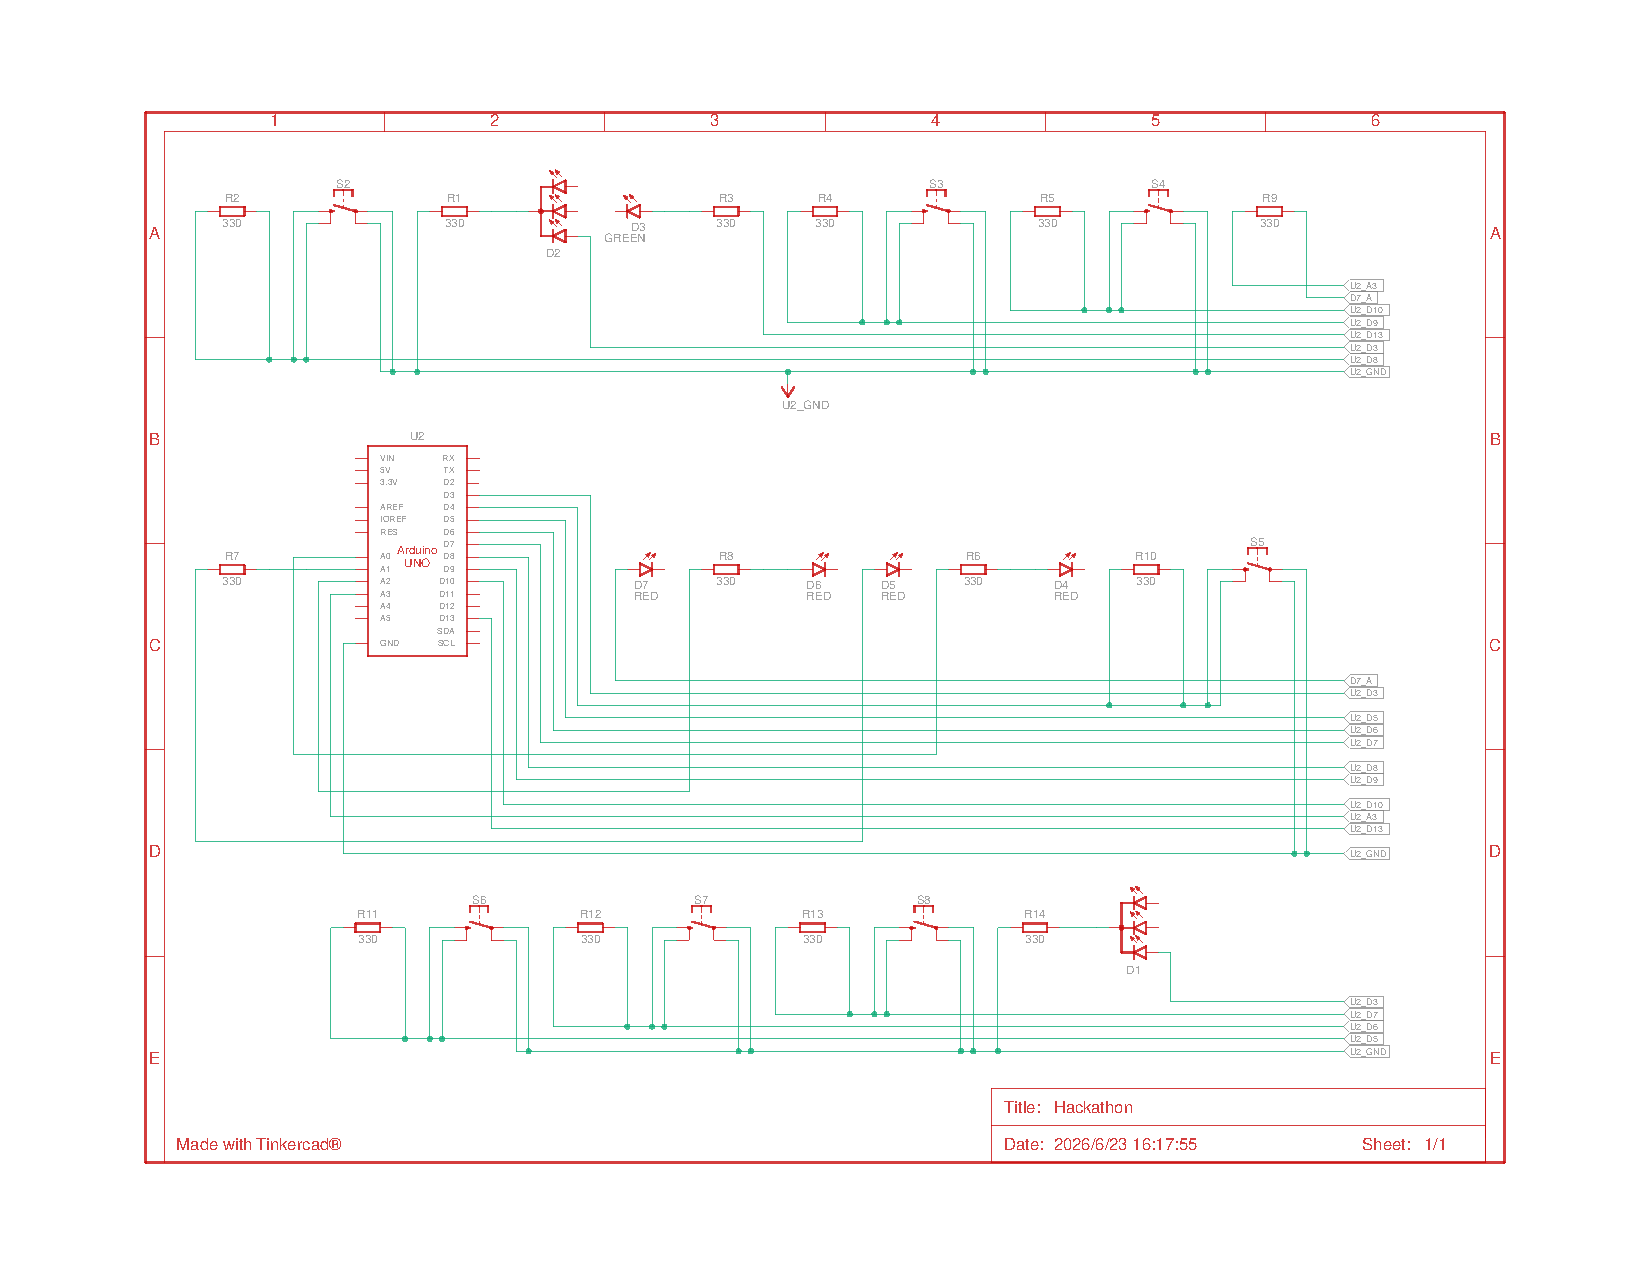
\includegraphics[width=0.95\textwidth]{circuit-diagram.pdf}
\caption{親機 hack-oya の回路図．D4--D7 子機ボタン群と D8 start ボタンを INPUT\_PULLUP で読み，A0--A3 の状態表示 LED を Arduino 側から駆動して点灯／消灯をトグル制御する．}
\label{fig:oya-schematic}
\end{figure}

\subsubsection{親機 hack-oya の回路実装イメージ}\label{sec:oya-photo}

図~\ref{fig:oya-photo} にブレッドボード上の実装イメージを示す．ボタンとボタンの隣接位置に状態表示 LED を物理的に配置することで，演奏者がどの子機を予約／参加させたかを目視で把握できる構成になっている．赤 LED 4 個がそれぞれ child0〜child3 のトグル状態を，緑 LED が tick 拍に合わせて点滅するインジケータ（D13）を表す．赤外線 LED は中央溝向こう側に配置し，D3 から駆動する．

\begin{figure}[H]
\centering
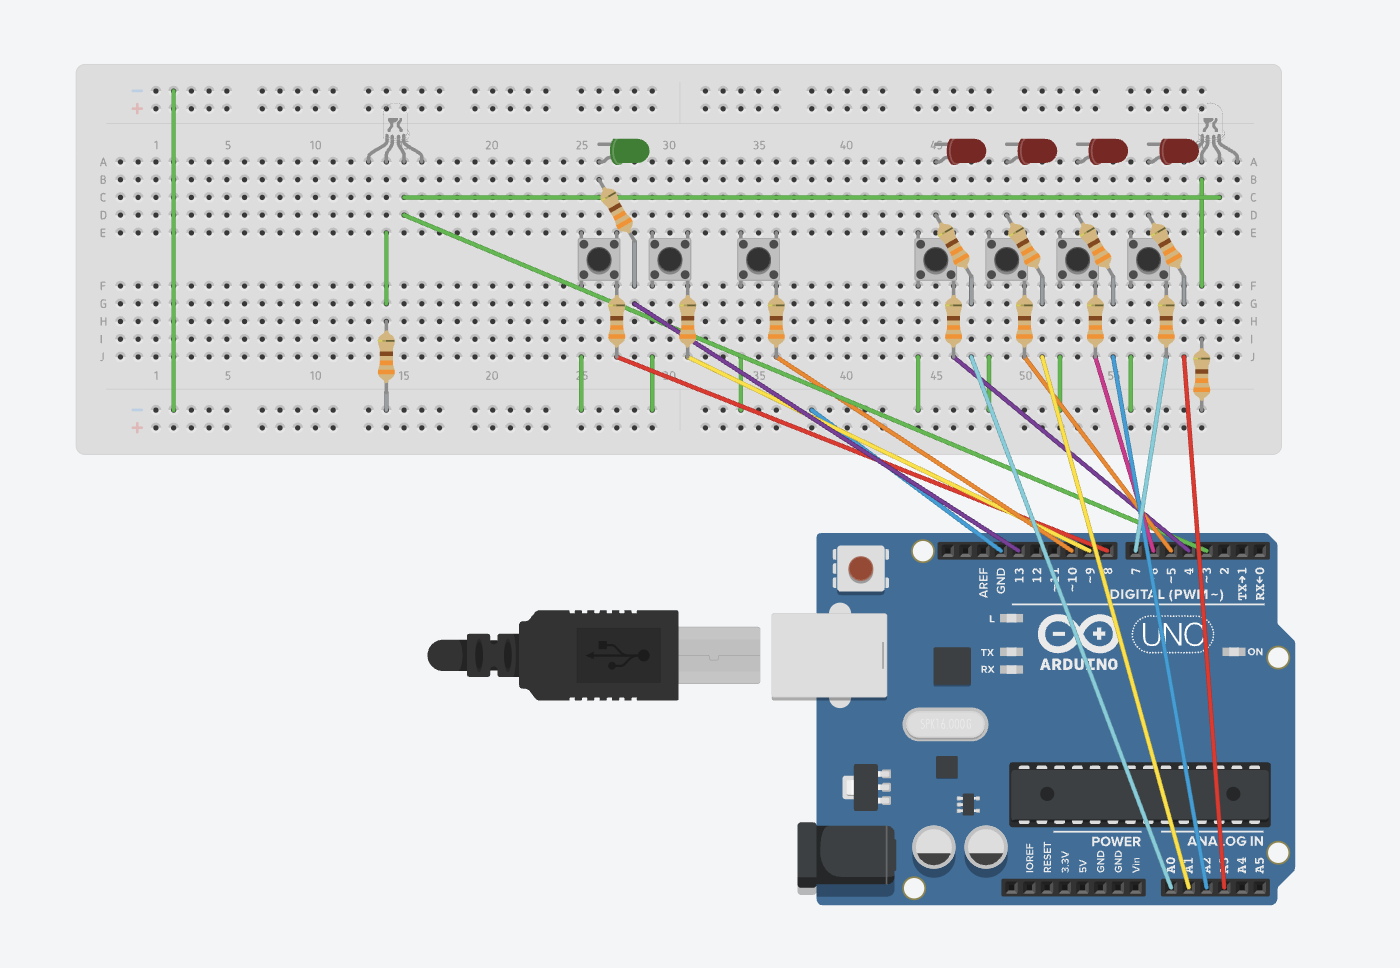
\includegraphics[width=0.95\textwidth]{image.png}
\caption{親機 hack-oya のブレッドボード実装イメージ．子機ボタン D4--D7 と隣接する A0--A3 トグル LED，start ボタン D8，IR LED（D3 駆動），動作確認用インジケータ LED（D13）が一枚のブレッドボードに収まる．}
\label{fig:oya-photo}
\end{figure}

なお，本週の回路組み立てと改修により親機は「演奏中の状態」と「どの子機を予約／参加させたか」の双方が物理 UI 上で同時に視認できるようになり，リハーサル中に Serial Monitor を確認することなく運用できるようになった．

\end{document}
